\documentclass[11pt,a4paper]{article}

\usepackage[utf8]{inputenc}
\usepackage[T1]{fontenc}
\usepackage[spanish,es-noshorthands,es-tabla]{babel}
\usepackage{lmodern}
\usepackage[margin=2.3cm]{geometry}
\usepackage{microtype}
\usepackage{amsmath,amssymb}
\usepackage{graphicx}
\usepackage{booktabs}
\usepackage{multirow}
\usepackage{xcolor}
\usepackage{subcaption}
\usepackage{tikz}
\usetikzlibrary{arrows.meta,positioning,fit,backgrounds}
\usepackage[style=numeric-comp,sorting=none,maxbibnames=6,backend=biber]{biblatex}
\usepackage{csquotes}
\usepackage[hidelinks]{hyperref}
\usepackage[spanish,noabbrev]{cleveref}
\addbibresource{refs.bib}

\decimalpoint
\newcommand{\Wn}{\mathrm{W}_1^{\mathrm{n}}}
\newcommand{\NNA}{\text{1-NNA}}

\title{Generación de árboles tropicales sintéticos a partir de modelos QSM reales:\\
comparación de tres familias de generadores y bosque virtual con LiDAR y cámara de profundidad en Isaac Sim}
\author{Nelson Broyer-Paco \and Angel Marquez-Aguilar \and Li Shi \and Josine \and Pacifique\\[2pt]\small Código y datos: \url{https://github.com/Nosl3n/Synthetic_Tree_G}}
\date{30 de octubre de 2026}

\begin{document}
\maketitle

\begin{abstract}
Los modelos de percepción para entornos forestales necesitan muchos datos 3D etiquetados, y estos son caros de obtener. Este trabajo estudia cómo generar árboles sintéticos realistas a partir de 201 modelos estructurales cuantitativos (QSM) de árboles tropicales escaneados con láser terrestre en Barro Colorado Island (Panamá), y cómo medir su parecido con los reales. Implementamos ocho generadores que cubren las tres familias de la literatura: (i) métodos que aprenden de árboles reales (perturbación, perturbación alométrica, recombinación de ramas, híbrido y un generador procedural que sortea reglas de ramas reales); (ii) un generador basado solo en reglas botánicas (alometría, filotaxis, perfiles de adelgazamiento); y (iii) un algoritmo clásico de crecimiento (\emph{space colonization}). Los evaluamos contra árboles reales no vistos mediante distancias de Wasserstein normalizadas sobre 22 rasgos de árbol y 10 de rama, un test de dos muestras por vecino más cercano (\NNA), una métrica de novedad y reglas de validez botánica. La recombinación de ramas de la misma especie es el método más fiel ($\NNA=56\%$ frente a $46\%$ entre reales), el generador procedural aprendido es el más novedoso entre los realistas, y su mezcla conserva la fidelidad de la recombinación aumentando la novedad de 0,73 a 1,19. Los generadores de reglas y de \emph{space colonization} producen árboles casi perfectamente distinguibles (89\% y 98\%). Finalmente, construimos un bosque virtual de 24 árboles sintéticos en NVIDIA Isaac Sim, con ramas modeladas como tubos continuos, en dos versiones: solo árboles (v1) y un bosque ambientado con terreno, sotobosque, madera muerta, rocas y árboles exteriores (v2). Un LiDAR rotatorio Ouster OS1 de 128 canales y una cámara RGB-D simulados generan datos etiquetados por clase a 10\,Hz, que se visualizan en tiempo real. En v2 el sotobosque supone el 21,7\,\% de los puntos LiDAR, una clase ausente en v1, mientras que la visibilidad de los troncos apenas cambia ($-4$\,\%).
\end{abstract}

\noindent\textbf{Palabras clave:} árboles sintéticos, QSM, LiDAR terrestre, modelado procedural inverso, evaluación de datos sintéticos, Isaac Sim, bosque tropical.

% =====================================================================
\section{Introducción}

La segmentación de nubes de puntos forestales (separar suelo, tronco, ramas y hojas, o individualizar árboles) es la base del inventario forestal automático y de la navegación de robots en cultivos y bosques. Las redes profundas que resuelven estas tareas, como PointNet++~\cite{qi2017pointnetpp}, necesitan grandes conjuntos etiquetados, y etiquetar nubes de puntos a mano es lento y caro. Por eso crece el interés en entrenar con datos sintéticos: modelos entrenados con árboles simulados igualan o superan a los entrenados con datos reales de otros sitios~\cite{bryson2023synthetic,bryson2024domain}, y el preentrenamiento sintético reduce drásticamente la cantidad de datos reales necesaria~\cite{she2026scaling}.

Sin embargo, la pregunta de \emph{cómo} generar los árboles sintéticos, y cómo saber si se parecen a los reales, está poco estudiada. La literatura de gráficos por ordenador evalúa árboles por su apariencia~\cite{polasek2021ictree,zhou2023deeptree}; la de teledetección evalúa los QSM por su error de volumen frente a medidas destructivas. Pocos trabajos comparan la \emph{estructura} (topología, ángulos, jerarquía de ramas) de árboles sintéticos con la de árboles reales usando métricas comunes.

Este trabajo aborda ese hueco con un conjunto público de 201 QSM de árboles tropicales~\cite{krishnamoorthy2022data}. Sus contribuciones son:
\begin{enumerate}
  \item Un \emph{pipeline} reproducible de lectura, limpieza y codificación local (tipo tortuga) de QSM que permite modificar, perturbar e injertar ramas reconstruyendo las uniones automáticamente.
  \item Ocho generadores que cubren las tres familias de la literatura: reglas, algoritmos de crecimiento y métodos que aprenden de árboles reales.
  \item Un protocolo de evaluación con separación estricta entrenamiento/prueba por árbol, que mide fidelidad, novedad y validez botánica, siempre con la referencia de la variabilidad real--real.
  \item Un bosque virtual en NVIDIA Isaac Sim~\cite{isaacsim} construido con los mejores generadores, con ramas continuas a partir de los QSM, en dos versiones (solo árboles y bosque ambientado). Incluye LiDAR y cámara de profundidad simulados, recopilación de datos etiquetados en ambas versiones y visualización en tiempo real.
\end{enumerate}

La \cref{fig:pipeline} resume el flujo completo.

\begin{figure}[t]
\centering
\begin{tikzpicture}[font=\footnotesize, >={Stealth[length=2mm]},
  box/.style={draw, rounded corners=2pt, align=center, minimum height=10mm, text width=31mm, fill=#1!12},
  box/.default=gray]
\node[box] (data) at (0,0) {201 QSM reales de BCI\\(Zenodo)};
\node[box] (prep) at (4.6,0) {Limpieza, topología\\y codificación local};
\node[box] (split) at (9.2,0) {Rasgos y partición\\152 \emph{train} / 49 \emph{test}};
\node[box=orange] (g1) at (0,-2.0) {Grupo 1: reglas\\G5};
\node[box=red] (g2) at (4.6,-2.0) {Grupo 2: algoritmo\\G6 (colonización)};
\node[box=blue] (g3) at (9.2,-2.0) {Grupo 3: aprenden de reales\\G0--G4};
\node[box=green] (eval) at (0,-4.5) {Evaluación frente a \emph{test}:\\$\Wn$, \NNA, novedad, validez};
\node[box=violet] (isaac) at (4.6,-4.5) {Bosque en Isaac Sim (G2+G4)\\LiDAR + cámara RGB-D};
\node[box=violet] (viz) at (9.2,-4.5) {Recopilación de datos\\y visor en tiempo real};
\draw[->] (data) -- (prep); \draw[->] (prep) -- (split);
\draw (split.south) -- ++(0,-0.25) coordinate (bus1);
\draw[->] (bus1) -| (g1.north); \draw[->] (bus1) -| (g2.north); \draw[->] (bus1) -- (g3.north);
\coordinate (bus2) at (0,-3.35);
\draw (g1.south) -- (bus2); \draw (g2.south) -- (4.6,-3.35); \draw (g3.south) -- (9.2,-3.35) -- (bus2);
\draw[->] (bus2) -- (eval.north);
\draw[->] (eval) -- (isaac); \draw[->] (isaac) -- (viz);
\end{tikzpicture}
\caption{Flujo del trabajo: de los QSM reales a los generadores, su evaluación y el bosque virtual con sensores.}
\label{fig:pipeline}
\end{figure}

% =====================================================================
\section{Trabajo relacionado}

Organizamos la literatura en tres familias de métodos, más la evaluación de datos sintéticos y su uso en percepción.

\paragraph{Reglas que cumplen los árboles reales.}
Hallé, Oldeman y Tomlinson describieron 23 \emph{modelos arquitecturales} que resumen cómo crecen los árboles, a partir precisamente de árboles tropicales~\cite{halle1978tropical}. La regla de Leonardo y el modelo de tubería postulan que el área de una rama madre se reparte entre sus hijas~\cite{shinozaki1964pipe}. La teoría metabólica (WBE) predice ramificaciones simétricas con exponentes fijos~\cite{west1997general,west1999plant}, pero en árboles tropicales escaneados las hijas son asimétricas y los exponentes se desvían~\cite{lau2019metabolic,yang2024treegraph}; solo los árboles dominantes del dosel se acercan a WBE~\cite{martinducup2020convergence}. En el mismo sitio de nuestros datos existen alometrías de altura y copa por especie, ajustadas con casi diez mil árboles~\cite{martinezcano2019allometry}.

\paragraph{Algoritmos que generan árboles.}
Los L-systems describen el crecimiento como reescritura de cadenas~\cite{lindenmayer1968mathematical,prusinkiewicz1990algorithmic}. AMAPsim~\cite{barczi2008amapsim} y GreenLab~\cite{yan2004greenlab} incorporan conocimiento botánico y reparto de recursos. En gráficos por ordenador, \emph{space colonization}~\cite{runions2007space} hace crecer las ramas hacia puntos libres de una envolvente, y los modelos autoorganizados~\cite{palubicki2009selforganizing} añaden competencia por luz entre yemas.

\paragraph{Métodos que aprenden de árboles reales.}
El modelado procedural inverso busca los parámetros de un generador que reproducen árboles de entrada; Šťava et al.~\cite{stava2014inverse} lo hacen con MCMC sobre árboles reconstruidos, y Guo et al.~\cite{guo2020inverse} infieren directamente las reglas de un L-system. Como complemento, Åkerblom et al.~\cite{akerblom2018leaf} insertan hojas sin intersecciones en QSM, y Treegraph~\cite{yang2024treegraph} extrae arquitectura de ramas a partir de nubes TLS.

\paragraph{Evaluación de datos sintéticos.}
La literatura de modelos generativos distingue fidelidad, diversidad y utilidad. Para fidelidad se usan tests de dos muestras basados en clasificadores~\cite{lopezpaz2017c2st}, en particular la precisión 1-NN \emph{leave-one-out} (\NNA), popularizada para nubes de puntos por PointFlow~\cite{yang2019pointflow}, y las métricas MMD/COV~\cite{achlioptas2018learning}. Para diversidad, la precisión y exhaustividad de variedades~\cite{kynkaanniemi2019precision}. La utilidad se mide entrenando con sintéticos y probando con reales (TSTR)~\cite{esteban2017rcgan}; van Breugel et al.~\cite{vanbreugel2023synthetic} advierten de que evaluar con datos del mismo generador sobreestima el rendimiento. Usamos además distancias de Wasserstein entre distribuciones de rasgos~\cite{ramdas2017wasserstein}. Para árboles, ICTree~\cite{polasek2021ictree} propone métricas perceptuales, y DeepTree~\cite{zhou2023deeptree} compara longitudes y número de ramas.

\paragraph{Datos sintéticos para percepción forestal.}
Bryson et al. entrenan PointNet++ con árboles sintéticos y obtienen un rendimiento comparable o superior al de datos reales de otros sitios~\cite{bryson2023synthetic}, y añaden adaptación de dominio para segmentar partes del árbol~\cite{bryson2024domain}. She et al.~\cite{she2026scaling} muestran que la simulación física del LiDAR (HELIOS++~\cite{winiwarter2022helios}) y la diversidad de escenas son los factores que más pesan (+37 y +39 puntos de F1), mientras que la cantidad de datos aporta menos (+5,5). En plantas industriales, simular el escaneo mejora el mIoU hasta un 7\%~\cite{noichl2024industrial}. La aleatorización de dominio~\cite{tobin2017domain} es la estrategia general para cerrar la brecha simulación--realidad.

\paragraph{Hueco.} No encontramos trabajos que ajusten generadores \emph{por especie} a estadísticas de QSM tropicales ni que comparen las tres familias con métricas estructurales comunes. Tampoco hay estudios que relacionen el parecido estructural de los sintéticos con su utilidad para entrenar redes.

% =====================================================================
\section{Datos}

\subsection{QSM de Barro Colorado Island}
Usamos el conjunto de Krishna Moorthy et al.~\cite{krishnamoorthy2022data} (CC BY 4.0): 201 árboles de 53 especies escaneados con láser terrestre en 2019 en Barro Colorado Island (Panamá) y reconstruidos con TreeQSM~2.4.0~\cite{raumonen2013treeqsm}. El estudio original evaluaba el efecto de las lianas, así que la selección de árboles no es aleatoria; anotamos esta condición como posible fuente de confusión. Cada QSM es una tabla de cilindros con inicio, eje, longitud, radio, padre y extensión (\cref{tab:datos}). El registro incluye además nubes de puntos separadas de madera y hoja.

\begin{table}[t]
\centering
\caption{Resumen de los 201 QSM reales (mediana [rango intercuartílico] salvo indicación).}
\label{tab:datos}
\begin{tabular}{lr}
\toprule
Árboles / especies & 201 / 53 \\
Altura (m), media $\pm$ d.e. & $28{,}5 \pm 5{,}1$ \\
Cilindros por árbol & 1785 [1115--3368] \\
Ramas por árbol & 366 [217--646] \\
Orden máximo de rama & 7 (3--10) \\
Radio de cilindro (cm) & 2,7 [1,6--3,7] \\
\bottomrule
\end{tabular}
\end{table}

\subsection{Limpieza y topología}\label{sec:limpieza}
Para cada árbol conservamos solo la parte conectada al cilindro raíz (en promedio se descarta el 0,56\% de los cilindros, que son fragmentos sueltos). La rama, el orden y la posición de cada cilindro se recalculan desde \texttt{parent} y \texttt{extension}; el resultado coincide al 100\% con TreeQSM en los 201 árboles, y el mismo código se aplica a reales y sintéticos.

Detectamos un artefacto de los datos reales: el 4,7\% de las uniones entre cilindros consecutivos de una misma rama tienen huecos de más de 20\,cm, en 199 de los 201 árboles. Son errores de reconstrucción de TreeQSM, no del procesamiento, y los generadores que copian geometría real los heredan.

\subsection{Partición entrenamiento/prueba}
Separamos por árbol, estratificando por especie: 152 árboles de entrenamiento (\emph{train}) y 49 de prueba (\emph{test}), con las especies de menos de tres árboles asignadas a \emph{train}. Todos los estadísticos de los generadores se ajustan solo con \emph{train}, y los sintéticos se generan solo a partir de árboles de \emph{train}. Los árboles de \emph{test} se usan únicamente para evaluar.

% =====================================================================
\section{Métodos}

\subsection{Codificación local de un QSM}
Para modificar un árbol sin romper sus uniones, expresamos cada cilindro $i$ en el marco ortonormal $F_p$ de su padre $p$, como una tortuga de L-system:
\begin{equation}
\mathbf{d}_i = F_p^{\top}(\mathbf{s}_i - \mathbf{s}_p), \qquad
(t_i, u_i, v_i) = \left(\frac{d_{i,z}}{\ell_p}, \frac{d_{i,x}}{r_p}, \frac{d_{i,y}}{r_p}\right), \qquad
\mathbf{a}_i^{\text{loc}} = F_p^{\top}\mathbf{a}_i ,
\end{equation}
donde $\mathbf{s}$ es el inicio, $\mathbf{a}$ el eje unitario, $\ell$ la longitud y $r$ el radio. El marco del hijo se obtiene aplicando a $F_p$ la rotación mínima que lleva $\mathbf{a}_p$ a $\mathbf{a}_i$ (forma de Rodrigues con el término $1/(1+c)$, numéricamente estable) y re-ortonormalizando en cada paso. La decodificación recorre el árbol en orden topológico. El error de ida y vuelta es de $\sim\!10^{-7}$\,m. Así, cambiar el radio, la longitud o el ángulo de una rama, o injertar un subárbol, desplaza automáticamente todo lo que cuelga de ella.

\subsection{Rasgos}
Con el mismo código para reales y sintéticos calculamos 22 rasgos de árbol (altura, DBH, volumen total, fracción de volumen en ramas, longitud total, número de ramas, orden máximo, ramas de orden 1 y 2, área y diámetro de copa por envolvente convexa, base de copa relativa, ángulo y cociente de diámetros medianos de las ramas de orden 1, densidad de hijas, regla de tubería, fracciones de volumen por orden y perfil de adelgazamiento del tronco a 30, 50, 70 y 90\% de su altura). También calculamos cinco rasgos por rama para los órdenes 1 y 2: ángulo de inserción, cociente de diámetros, cociente de longitudes, cenit y densidad de hijas.

En \emph{train} medimos las reglas que usan los generadores:
\begin{itemize}
  \item alometría de árbol $H \propto \text{DBH}^{0{,}427}$;
  \item alometría de rama $\ell \propto r^{0{,}345}$ (residuo d.e.\ 0,79 en escala log);
  \item variabilidad natural del cociente de diámetros (d.e.\ log de 0,73 en orden 1 a 1,0 en orden 7);
  \item variabilidad del ángulo de inserción (d.e.\ de 40° en orden 1 a 32° en orden 8);
  \item exponente de Leonardo $\Delta$ tal que $r_p^{\Delta} = \sum_c r_c^{\Delta}$: mediana $\Delta = 2{,}38$ sobre 25\,728 bifurcaciones con $r_p > 2$\,cm, cerca del valor clásico 2.
\end{itemize}

\subsection{Generadores}
Cada generador produce cinco árboles por árbol de \emph{train} (760 en total). Los resumimos en la \cref{tab:gen}.

\begin{table}[t]
\centering
\caption{Generadores implementados. Del árbol fuente, cada generador toma lo que indica la última columna.}
\label{tab:gen}
\small
\begin{tabular}{clp{7.1cm}p{2.9cm}}
\toprule
Grupo & Generador & Idea & Toma del fuente \\
\midrule
3 & G0 \texttt{iid\_radius} & Radio de cada cilindro $\times\,U(0{,}9;1{,}1)$, línea base del repositorio \texttt{qsm-variation}. & Todo \\
3 & G1 \texttt{allometric} & Por rama: factores log-normales de media 1 en radio y longitud (ligada por la alometría), y ruido en ángulo de inserción y azimut; magnitud $\alpha\times$ variabilidad natural; escala global $H\propto\text{DBH}^{b}$. & Todo \\
3 & G2 \texttt{recombine} & Cada rama de orden 1 se sustituye con $p=0{,}5$ por la de otro árbol de \emph{train} de la misma especie, con altura relativa ($\pm0{,}15$) y grosor ($\times0{,}5$--2) parecidos; radio $\times k$, longitud $\times k^{b}$. & Tronco, resto de ramas \\
3 & G3 \texttt{hybrid} & G2 seguido de G1 con $\alpha=0{,}25$. & Tronco, resto de ramas \\
3 & G4 \texttt{procedural} & Árbol nuevo rama a rama: cada rama sortea la \enquote{regla} completa de una rama real de la misma especie y orden (posición, cociente de diámetros, ángulos, curvatura, perfil de radio, residuo de longitud, n.º de hijas), entre ramas cuyo padre real tenía grosor parecido. & Especie, tamaño y perfil del tronco, n.º de ramas de orden 1 \\
1 & G5 \texttt{rules} & Árbol nuevo solo con medias y dispersiones por especie y orden: alometrías, perfil de adelgazamiento medio, filotaxis de 137,5°, ángulos, cenit, densidad de ramas y cociente de longitudes hija/madre $\le$ percentil 95. & Especie, DBH \\
2 & G6 \texttt{colonization} & \emph{Space colonization}~\cite{runions2007space} en un elipsoide de copa; radios por la regla de Leonardo con $\Delta=2{,}38$ ajustada al DBH. & Especie, envolvente de copa, longitud total \\
\bottomrule
\end{tabular}
\end{table}

\paragraph{G1, perturbación alométrica.} Para cada rama $b$ de orden $o$, con $\sigma_r = \alpha\,\sigma_{\text{ratio},o}$ y $\sigma_\ell = \alpha\,\sigma_{\text{res},\ell}$:
\begin{equation}
r' = r\, e^{\varepsilon_r - \sigma_r^2/2}, \quad
\ell' = \ell\, e^{\,b\,(\varepsilon_r + \sigma_r^2/2) + \varepsilon_\ell - (b^2\sigma_r^2 + \sigma_\ell^2)/2}, \quad
\theta' = \theta + \alpha\,\sigma_{\theta,o}\,\xi ,
\end{equation}
con $\varepsilon_r \sim \mathcal{N}(0,\sigma_r^2)$, $\varepsilon_\ell \sim \mathcal{N}(0,\sigma_\ell^2)$ y $\xi \sim \mathcal{N}(0,1)$. Los términos de corrección mantienen la media; sin ellos, el ruido log-normal infla el tamaño del árbol. Además se impone que una rama no supere el radio de su padre, salvo que ya lo hiciera en el original.

\paragraph{G2, recombinación.} Si el grosor de la rama sustituida es $r_t$ y el de la donante $r_d$, la donante se reescala con $k = r_t/r_d$: radios $\times k$ y longitudes $\times k^{b}$, con $b=0{,}345$. Conserva su ángulo de inserción y adopta el azimut de la rama sustituida. En especies con un solo árbol en \emph{train} se usan donantes de otras especies, lo que afecta al 16\% de los sintéticos.

\paragraph{G4, procedural aprendido.} Es una versión sin ajuste inverso del enfoque de Šťava et al.~\cite{stava2014inverse}. En lugar de muestrear cada parámetro por separado, lo que rompe sus correlaciones, se sortea la fila completa de una rama real. Para evitar aplicar la regla de una rama fina sobre un padre grueso, se toman 32 candidatas al azar y se elige entre las 3 cuyo padre real tenía el grosor más parecido. La curvatura se impone interpolando (\emph{slerp}) entre la dirección inicial y la final de la rama real, más una ondulación con la misma amplitud media medida en las uniones reales.

\paragraph{G5, reglas.} Al principio aplicamos Leonardo en cada lateral para adelgazar los ejes, pero el tronco quedaba casi sin grosor (radio a media altura del 9\% del de 1,3\,m). En los QSM, la suma de áreas de las hijas \emph{supera} la de la madre (mediana del cociente 1,34), así que G5 usa el perfil de adelgazamiento medio de la especie, y reservamos Leonardo para G6.

\paragraph{G6, space colonization.} Los puntos de atracción se distribuyen uniformemente en un elipsoide con la altura, la base y el diámetro de copa del fuente, en número proporcional a su longitud total (un punto por metro). El radio de influencia es tres veces la separación media entre puntos, la distancia de eliminación es 0,5\,m, el segmento mide 0,25\,m y hay un tropismo vertical de 0,15. Los radios siguen $r = r_{\text{tip}}\,w^{1/\Delta}$, donde $w$ es el número de puntas aguas abajo, ajustado al DBH.

Los únicos parámetros elegidos a mano fueron la ondulación de G4 y la densidad de puntos de G6. Comprobamos que la elección es la misma usando medianas de \emph{train} o de \emph{test}, de modo que no hay fuga de información hacia la evaluación.

\subsection{Métricas}
Sean $\mathcal{S}$ los sintéticos y $\mathcal{T}$ los árboles de \emph{test}. Todas las métricas se reportan junto a la referencia real--real, que compara \emph{train} con \emph{test}: un sintético es \enquote{tan real como lo real} si su distancia a \emph{test} se parece a la de \emph{train} a \emph{test}.

\paragraph{Wasserstein normalizada.} Para cada rasgo $j$ (en escala logarítmica los de tamaño):
\begin{equation}
\Wn(j) = \frac{W_1\!\left(F_j^{\mathcal{S}}, F_j^{\mathcal{T}}\right)}{\sigma_j^{\text{real}}}.
\end{equation}

\paragraph{\NNA.} Con los vectores de rasgos estandarizados, se juntan $|\mathcal{T}|=49$ árboles de test y 49 sintéticos al azar, y se mide la precisión \emph{leave-one-out} de un clasificador 1-NN que predice si un árbol es real o sintético~\cite{lopezpaz2017c2st,yang2019pointflow}. Un 50\% significa indistinguible. Promediamos 50 submuestreos y, para las mezclas, 5 semillas.

\paragraph{Novedad.} Mide si un sintético es un árbol distinto o una copia de su fuente:
\begin{equation}
\text{novedad} = \frac{\operatorname{med}_{s\in\mathcal{S}} \lVert \mathbf{z}_s - \mathbf{z}_{\text{fuente}(s)} \rVert}{\operatorname{med}_{i\in\text{train}} \min_{j\neq i} \lVert \mathbf{z}_i - \mathbf{z}_j\rVert}.
\end{equation}
Vale 0 para una copia y 1 si el sintético se aleja de su fuente lo mismo que un árbol real de su vecino real más cercano.

\paragraph{Validez botánica.} Porcentaje de ramas más gruesas que su madre y mediana de la regla de tubería $\sum r_c^2/r_p^2$.

% =====================================================================
\section{Resultados}

\subsection{Comparación de generadores}
La \cref{tab:res} y la \cref{fig:fn} muestran los resultados, y la \cref{fig:arboles} un ejemplo visual.

\begin{table}[t]
\centering
\caption{Evaluación frente a los 49 árboles de \emph{test} (760 sintéticos por generador). En negrita, el mejor valor entre los sintéticos.}
\label{tab:res}
\small
\setlength{\tabcolsep}{4pt}
\begin{tabular}{lccccccccc}
\toprule
 & Real & G0 & G1 & G1 & G2 & G3 & G4 & G5 & G6 \\
 & (ref.) & & $\alpha$=0,25 & $\alpha$=0,5 & & & & & \\
\midrule
Grupo & -- & 3 & 3 & 3 & 3 & 3 & 3 & 1 & 2 \\
\NNA{} (\%) $\downarrow$ & 45,5 & \textbf{54,2} & 57,0 & 65,1 & 55,9 & 55,9 & 63,2 & 89,2 & 97,8 \\
Novedad & 1,00 & 0,31 & 0,38 & 0,72 & 0,73 & 0,81 & 1,60 & 1,98 & 2,13 \\
$\Wn$ árbol (media) $\downarrow$ & 0,202 & \textbf{0,201} & 0,226 & 0,310 & 0,209 & 0,233 & 0,300 & 0,632 & 0,820 \\
$\Wn$ rama (media) $\downarrow$ & 0,039 & \textbf{0,042} & 0,052 & 0,075 & 0,049 & 0,061 & 0,063 & 0,096 & 0,312 \\
Ramas $>$ madre (\%) & 5,8 & 12,0 & 5,1 & 5,2 & 5,7 & 5,0 & 5,5 & 0,0 & 0,0 \\
Tubería (mediana) & 1,34 & 1,35 & 1,33 & 1,30 & 1,34 & 1,33 & 1,38 & 1,21 & 1,10 \\
\bottomrule
\end{tabular}
\end{table}

\begin{figure}[t]
\centering
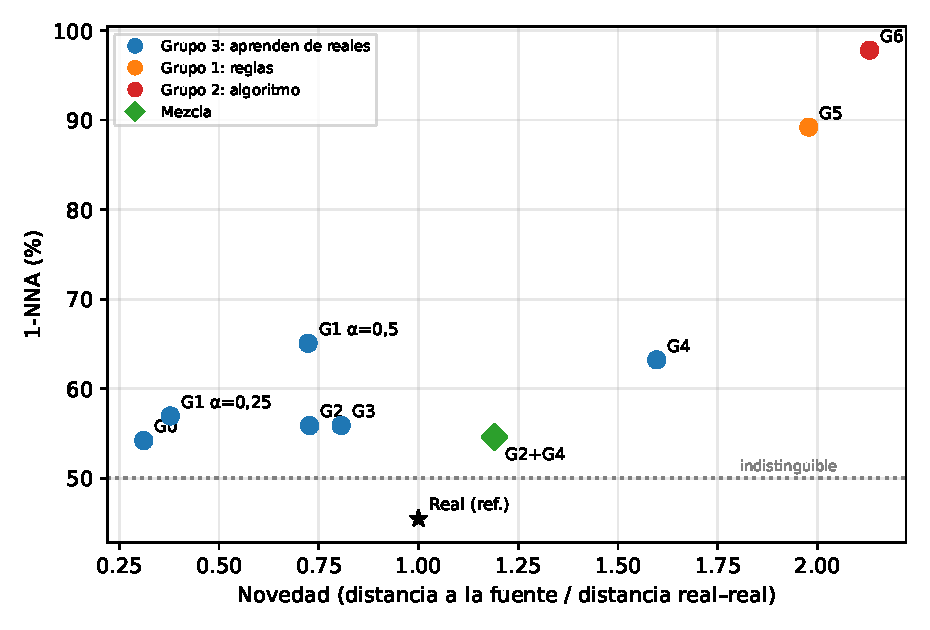
\includegraphics[width=0.72\linewidth]{figs/fidelidad_novedad.pdf}
\caption{Fidelidad (\NNA, más bajo es mejor; 50\% = indistinguible) frente a novedad. La estrella es la referencia real--real. Cuanto menos se apoya un método en ramas reales, más novedoso es y menos se parece a lo real.}
\label{fig:fn}
\end{figure}

\begin{figure}[t]
\centering
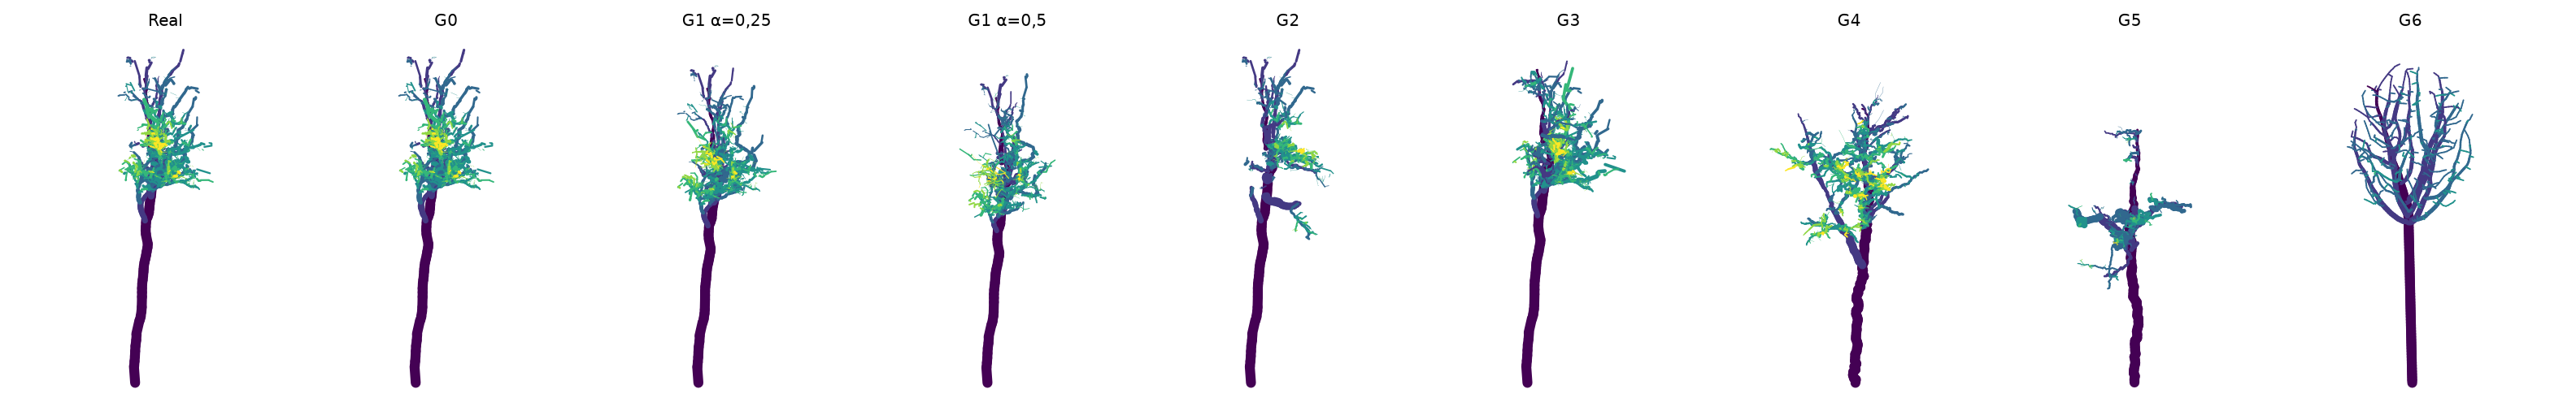
\includegraphics[width=\linewidth]{figs/generadores.png}
\caption{Árbol real (\emph{Trichilia tuberculata}, TRITUB\_213134) y un sintético de cada generador, en vista lateral. El color indica el orden de rama.}
\label{fig:arboles}
\end{figure}

Lo más relevante:
\begin{itemize}
  \item \textbf{G0} tiene la menor distancia porque es casi una copia (novedad 0,31), y además \emph{duplica} el porcentaje de ramas más gruesas que su madre (12\% frente a 5,8\%). Rompe una regla botánica básica sin crear árboles nuevos.
  \item \textbf{G1} muestra el compromiso fidelidad--novedad. Con $\alpha=0{,}5$ la copa se ensancha un 22\%, porque el ruido independiente por rama no conoce la forma global de la copa.
  \item \textbf{G2} es el mejor equilibrio: novedad 0,73 con $\Wn$ de árbol (0,209) casi igual a la referencia real (0,202).
  \item \textbf{G4} es el único generador realista que crea árboles realmente nuevos (novedad 1,60). Sus errores principales son el reparto de volumen entre órdenes y el número de ramas de orden 2 (\cref{fig:w1}).
  \item \textbf{G5} acierta el tamaño (altura, DBH, copa), pero tiene un tercio de las ramas (128 frente a 365) y menos órdenes (5 frente a 7). Las reglas medias, aplicadas por separado, no reproducen la ramificación densa y desordenada de los QSM.
  \item \textbf{G6} acierta la longitud total y la copa, que fija la envolvente, pero produce una arquitectura de gráficos por ordenador: jerarquía poco profunda (orden máximo 4), tronco sin adelgazar y ramas en abanico.
\end{itemize}

\begin{figure}[t]
\centering
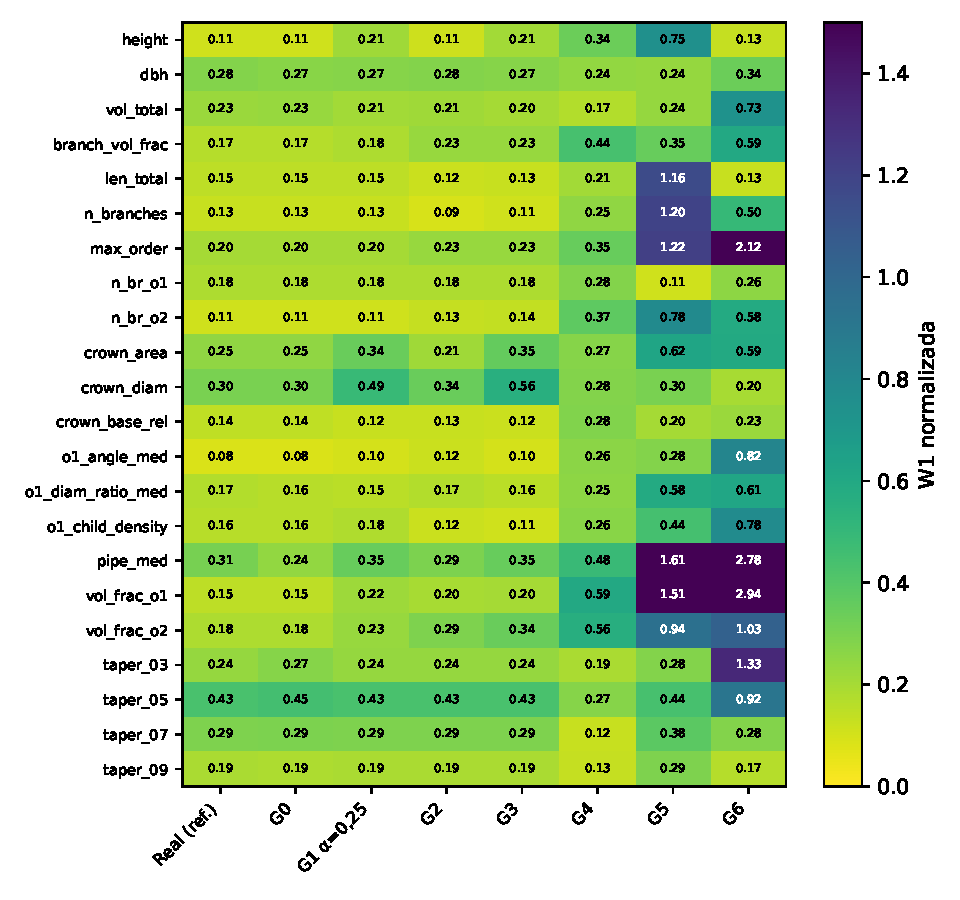
\includegraphics[width=0.66\linewidth]{figs/w1_rasgos.pdf}
\caption{Distancia de Wasserstein normalizada por rasgo de árbol frente a \emph{test}. La primera columna es la referencia real--real.}
\label{fig:w1}
\end{figure}

\subsection{Combinaciones de generadores}
Mezclamos generadores a partes iguales, manteniendo 760 árboles en total (\cref{tab:mix}). La mezcla G2+G4 tiene la misma fidelidad que G2 solo ($54{,}6 \pm 1{,}0\%$ frente a $54{,}5 \pm 0{,}5\%$; la diferencia está dentro del ruido entre semillas), pero su novedad es mucho mayor (1,19 frente a 0,73). Añadir G3 no aporta nada, y mezclar con G5 o G6 degrada la fidelidad.

\begin{table}[t]
\centering
\caption{Mezclas de generadores (760 árboles, partes iguales). Media de 5 semillas (submuestreos distintos); para \NNA, media $\pm$ d.e.}
\label{tab:mix}
\begin{tabular}{lccc}
\toprule
Conjunto & \NNA{} (\%) & Novedad & $\Wn$ árbol \\
\midrule
Real \emph{train} (ref.) & $47{,}5 \pm 0{,}4$ & 1,00 & 0,20 \\
G2 & $54{,}5 \pm 0{,}5$ & 0,73 & 0,21 \\
G4 & $60{,}7 \pm 1{,}4$ & 1,60 & 0,30 \\
\textbf{G2 + G4} & $\mathbf{54{,}6 \pm 1{,}1}$ & \textbf{1,19} & 0,23 \\
G2 + G3 + G4 & $54{,}8 \pm 1{,}1$ & 1,01 & 0,23 \\
G2 + G5 & $64{,}1 \pm 0{,}6$ & 1,41 & 0,36 \\
G2 + G6 & $67{,}7 \pm 0{,}9$ & 1,66 & 0,47 \\
\bottomrule
\end{tabular}
\end{table}

% =====================================================================
\section{Bosque virtual con sensores en Isaac Sim}

Con la mejor combinación (G2+G4) construimos un bosque virtual para generar datos de sensores, que es el paso necesario para medir la utilidad de los sintéticos (TSTR). Construimos dos versiones del mismo bosque, con los mismos árboles, posiciones y recorrido:
\begin{itemize}
  \item \textbf{v1, solo árboles:} los 24 árboles sobre suelo plano y cielo de campo;
  \item \textbf{v2, bosque ambientado:} los mismos árboles, con terreno, sotobosque, madera muerta, rocas y un anillo exterior de árboles.
\end{itemize}
Así las diferencias entre los datos de ambas se deben solo a la ambientación.

\subsection{Árboles: de cilindros a ramas continuas}
Elegimos 12 árboles G2 y 12 G4 con fuentes distintas y los colocamos en una parcela de $60\times60$\,m mediante muestreo de disco de Poisson (separación mínima de 7\,m) con rotación aleatoria.

Una primera versión convertía cada cilindro QSM en un tubo independiente. El resultado era visualmente pobre: se veían los cilindros, y los huecos de TreeQSM (\cref{sec:limpieza}) dejaban ramas desconectadas. La versión final construye \textbf{un tubo continuo por rama}:
\begin{enumerate}
  \item El eje de la rama une el inicio del primer cilindro, el punto medio de cada unión (lo que cierra los huecos) y el final del último.
  \item Cada rama hija empieza en el punto del eje de su madre más cercano a su base, así que nace desde dentro de ella.
  \item El eje se alisa con un filtro laplaciano~\cite{taubin1995signal}, con más iteraciones cuanto más gruesa es la rama (entre 1 y 12, $\propto r/2$\,cm), lo que elimina el zigzag de reconstrucción de los troncos sin cambiar la forma de las ramas finas. Después se suaviza con dos iteraciones de Chaikin~\cite{chaikin1974curve}.
  \item Los anillos de vértices (de 6 a 20 lados según el radio) se orientan con marcos de transporte paralelo~\cite{bishop1975frame}, que evitan la torsión, y se comparten entre segmentos consecutivos.
  \item Cada rama tiene normales suaves y coordenadas UV a lo largo de su longitud, de modo que la corteza sigue su dirección. La punta se cierra en cono.
\end{enumerate}
Cada árbol tiene una malla de tronco (orden 0) y otra de ramas, etiquetadas semánticamente (\texttt{trunk}, \texttt{branch}). El bosque v1 suma 2,36\,M caras en formato OpenUSD~\cite{pixarusd}. Los materiales son PBR con texturas escaneadas de corteza~\cite{polyhaven}.

\subsection{Ambientación de bosque (v2)}
Para dar sensación de bosque añadimos los siguientes elementos, todos con recursos CC0 de Poly Haven~\cite{polyhaven}:
\begin{itemize}
  \item \textbf{Terreno:} suma de 14 ondas de 12 a 90\,m de longitud (desnivel de 2,4\,m en la parcela; d.e.\ 0,49\,m), con textura de hojarasca. Los árboles y la plataforma siguen su altura.
  \item \textbf{Horizonte de bosque:} un anillo de 110 árboles sintéticos G2/G4 adicionales, de fuentes no usadas en la parcela, entre 34 y 95\,m del centro, en una versión ligera de la malla (mitad de lados y sin ramitas de menos de 6\,mm). Lo completa un cielo HDRI de sendero de selva.
  \item \textbf{Sotobosque} en un radio de 60\,m: 4\,431 plantas (helechos, \emph{Calathea}, \emph{Anthurium} y arbustos).
  \item \textbf{Madera muerta:} 835 objetos (tocones, troncos caídos, raíces, corteza y ramas secas).
  \item \textbf{Rocas:} 23 rocas con musgo.
\end{itemize}
Las plantas y los objetos se instancian (\emph{PointInstancer}) y se etiquetan como \texttt{understory}, \texttt{deadwood} y \texttt{rock}. Ninguno se coloca sobre el recorrido de la plataforma. La parte no instanciada de v2 suma 5,40\,M caras. La \cref{fig:vistas} compara ambas versiones.

\begin{figure}[t]
\centering
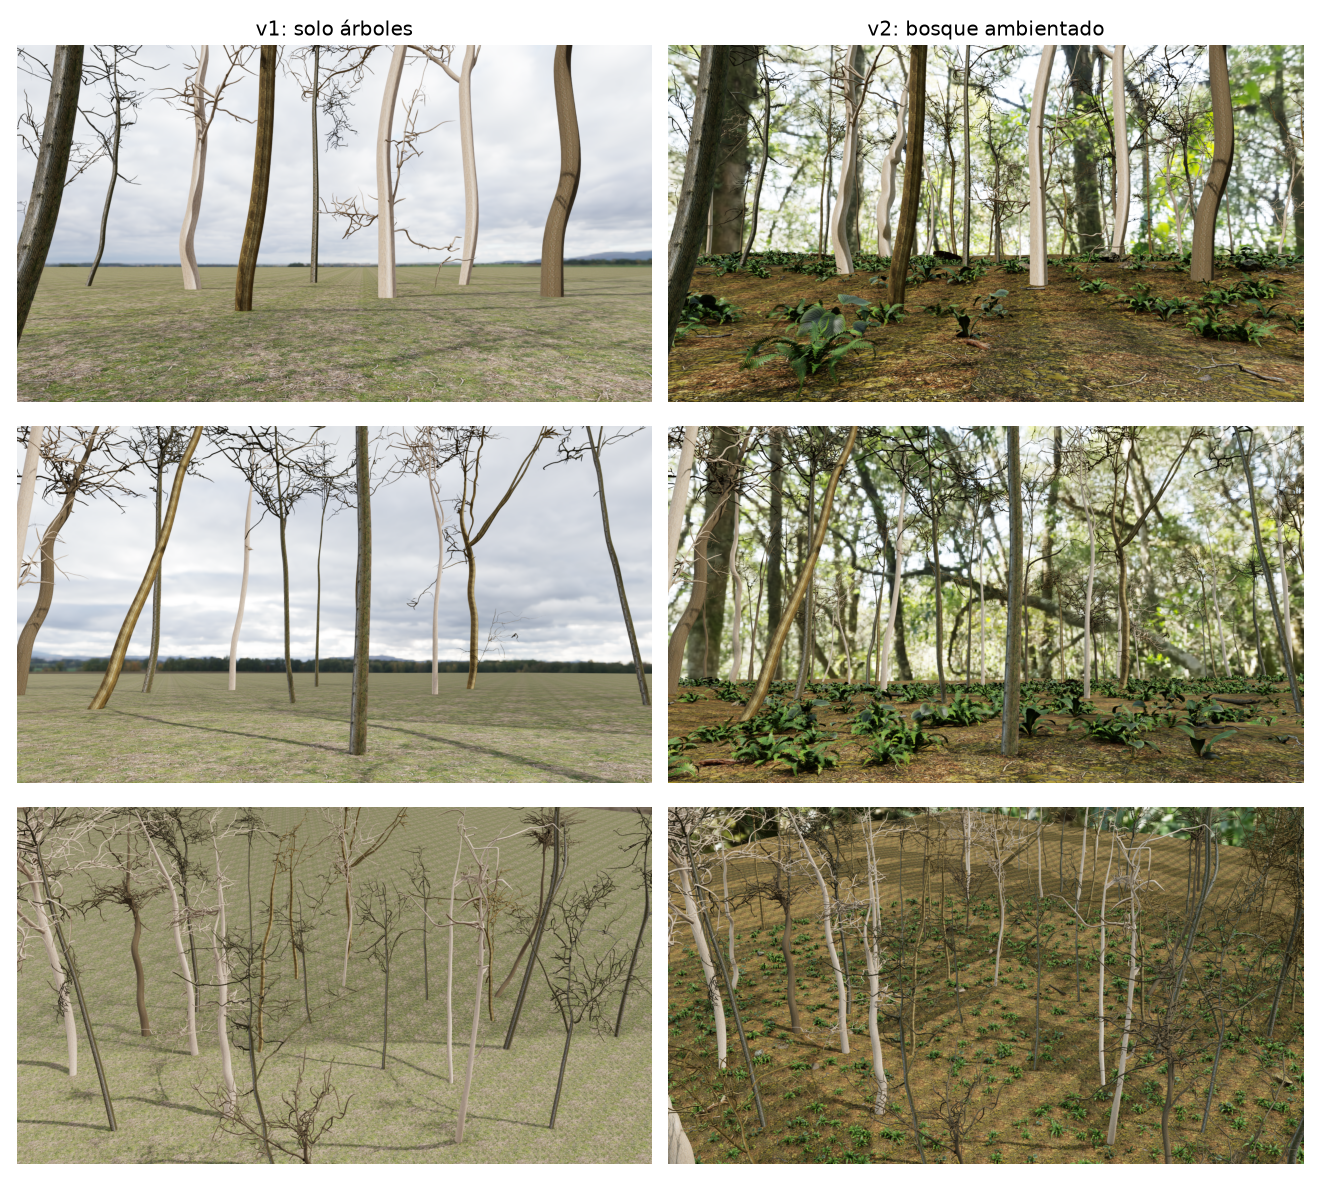
\includegraphics[width=0.92\linewidth]{figs/vistas_v1_v2.png}
\caption{El mismo bosque en Isaac Sim: v1, solo árboles (izquierda), y v2, bosque ambientado (derecha). Arriba, vista desde el recorrido de la plataforma; en medio, a la altura de una persona; abajo, vista aérea.}
\label{fig:vistas}
\end{figure}

\subsection{Sensores}
Una plataforma recorre a 1\,m/s un circuito cerrado de 83\,m, de la forma $r(\theta) = r_0 + A\sin(k\theta+\varphi)$. Sus parámetros se eligen para pasar cerca de los árboles sin acercarse a menos de 2,5\,m de ningún tronco. La plataforma lleva dos sensores:
\begin{itemize}
  \item \textbf{LiDAR rotatorio} Ouster OS1 (REV6, 128 canales, 1024 columnas, 10\,Hz)~\cite{ousteros1} a 1,8\,m del suelo, simulado con el trazado de rayos RTX de Isaac Sim 6.2~\cite{isaacsim}. Cada barrido se decodifica de coordenadas esféricas (acimut, elevación, rango) a cartesianas y se transforma a coordenadas de mundo. Mediante el identificador de objeto de cada retorno, cada punto recibe su clase y su árbol.
  \item \textbf{Cámara RGB-D} a 1,2\,m con la óptica de una Intel RealSense D455 (87° de campo horizontal, $848\times480$)~\cite{realsensed455}: RGB, profundidad al plano imagen y segmentación semántica.
\end{itemize}

\subsection{Recopilación y visualización}
A 10\,Hz, cada fotograma (último barrido LiDAR, imágenes, poses de plataforma, LiDAR y cámara, e intrínsecos) se guarda en un archivo comprimido con escritura atómica. Un proceso independiente, basado en Rerun~\cite{rerun}, lee los fotogramas según aparecen y los muestra en tiempo real. La vista 3D incluye:
\begin{itemize}
  \item el barrido actual coloreado por clase;
  \item el mapa acumulado submuestreado por vóxeles de 15\,cm;
  \item el esqueleto \enquote{verdad} de cada árbol;
  \item la trayectoria y la cámara con su profundidad proyectada.
\end{itemize}
También hay vistas 2D de RGB, profundidad y segmentación, y series temporales de puntos por clase. El mismo visor reproduce grabaciones, lo que sirve como respaldo para una demostración.

\subsection{Resultados: datos de v1 y v2}
Grabamos una vuelta completa (84\,s simulados, 840 fotogramas) en cada versión, en una RTX 5070 Ti (\cref{tab:v1v2}, \cref{fig:sens,fig:lidarv}).

\begin{table}[t]
\centering
\caption{Datos de sensores en una vuelta completa por las dos versiones del bosque (mismos árboles y mismo recorrido).}
\label{tab:v1v2}
\small
\begin{tabular}{lrr}
\toprule
 & v1: solo árboles & v2: bosque ambientado \\
\midrule
Tiempo real por vuelta (84\,s simulados) & 144\,s (0,58$\times$) & 196\,s (0,43$\times$) \\
Tamaño de la grabación & 1,7\,GB & 2,6\,GB \\
Puntos LiDAR por barrido & $60\,098 \pm 1\,166$ & $77\,823 \pm 917$ \\
\addlinespace
\multicolumn{3}{l}{\emph{LiDAR, \% de puntos}} \\
\quad suelo & 83,0 & 52,0 \\
\quad tronco & 15,8 & 17,7 \\
\quad rama & 1,3 & 7,2 \\
\quad sotobosque & -- & 21,7 \\
\quad madera muerta & -- & 1,3 \\
\quad roca & -- & 0,2 \\
\addlinespace
\multicolumn{3}{l}{\emph{Cámara, \% de píxeles}} \\
\quad cielo / fondo & 45,1 & 36,2 \\
\quad suelo & 47,5 & 40,1 \\
\quad tronco & 6,6 & 9,2 \\
\quad rama & 0,8 & 4,8 \\
\quad sotobosque & -- & 9,0 \\
\quad madera muerta + roca & -- & 0,7 \\
\addlinespace
Árboles de la parcela vistos por barrido (de 24) & 23,9 & 23,8 \\
Puntos de tronco por árbol de la parcela visto & 398 & 382 ($-4\%$) \\
Error del suelo LiDAR frente al terreno (mediana) & 1\,mm & 4\,mm \\
Distancia mínima del LiDAR a un objeto & 1,76\,m & 1,73\,m \\
\bottomrule
\end{tabular}
\end{table}

\begin{figure}[t]
\centering
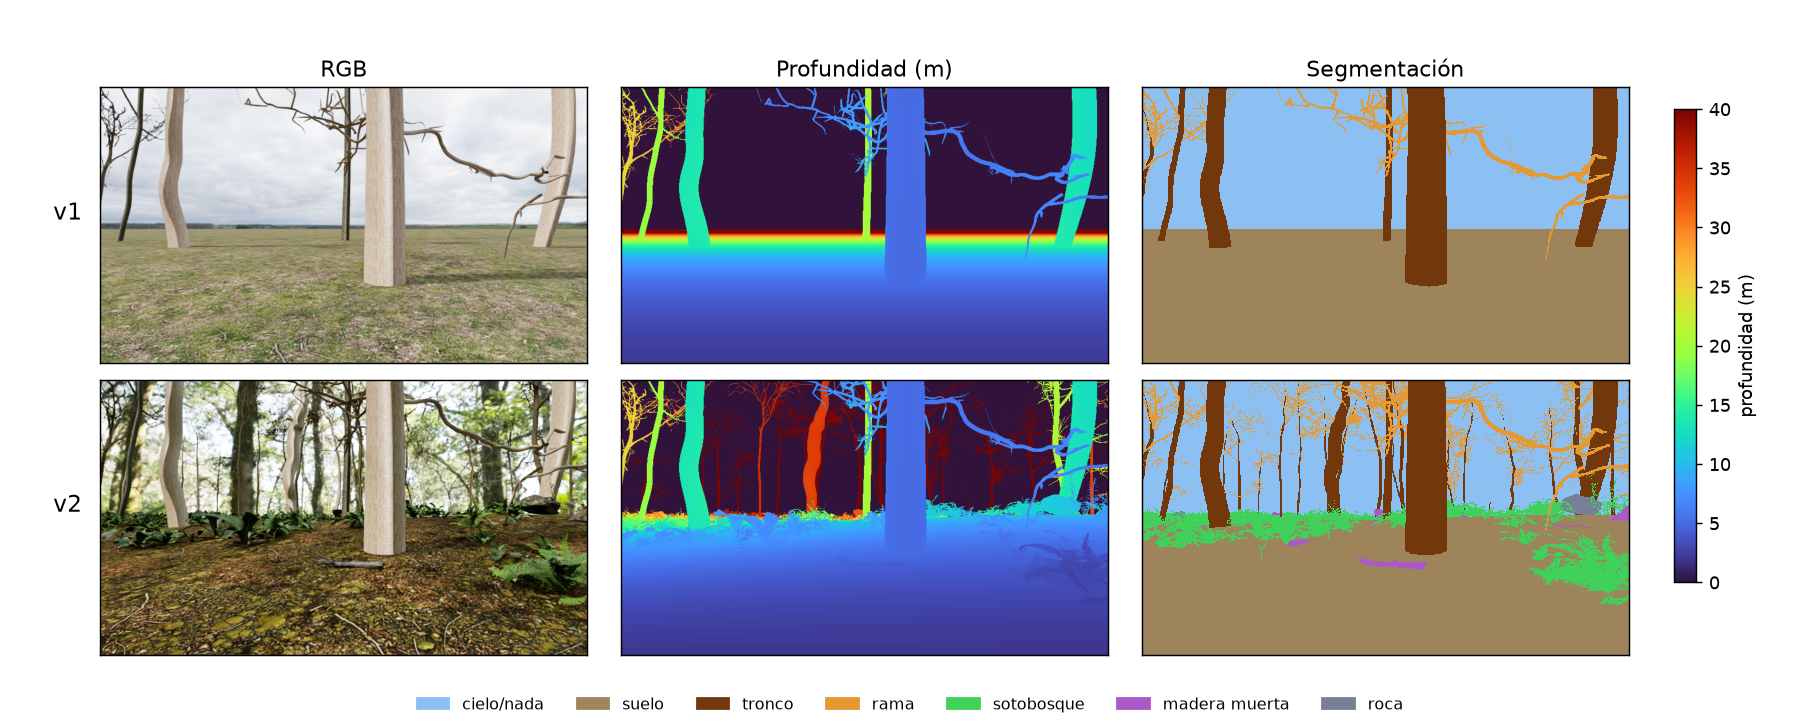
\includegraphics[width=\linewidth]{figs/sensores_v1_v2.png}
\caption{Cámara RGB-D en el mismo instante y la misma pose en v1 (arriba) y v2 (abajo): RGB, profundidad y segmentación semántica.}
\label{fig:sens}
\end{figure}

\begin{figure}[t]
\centering
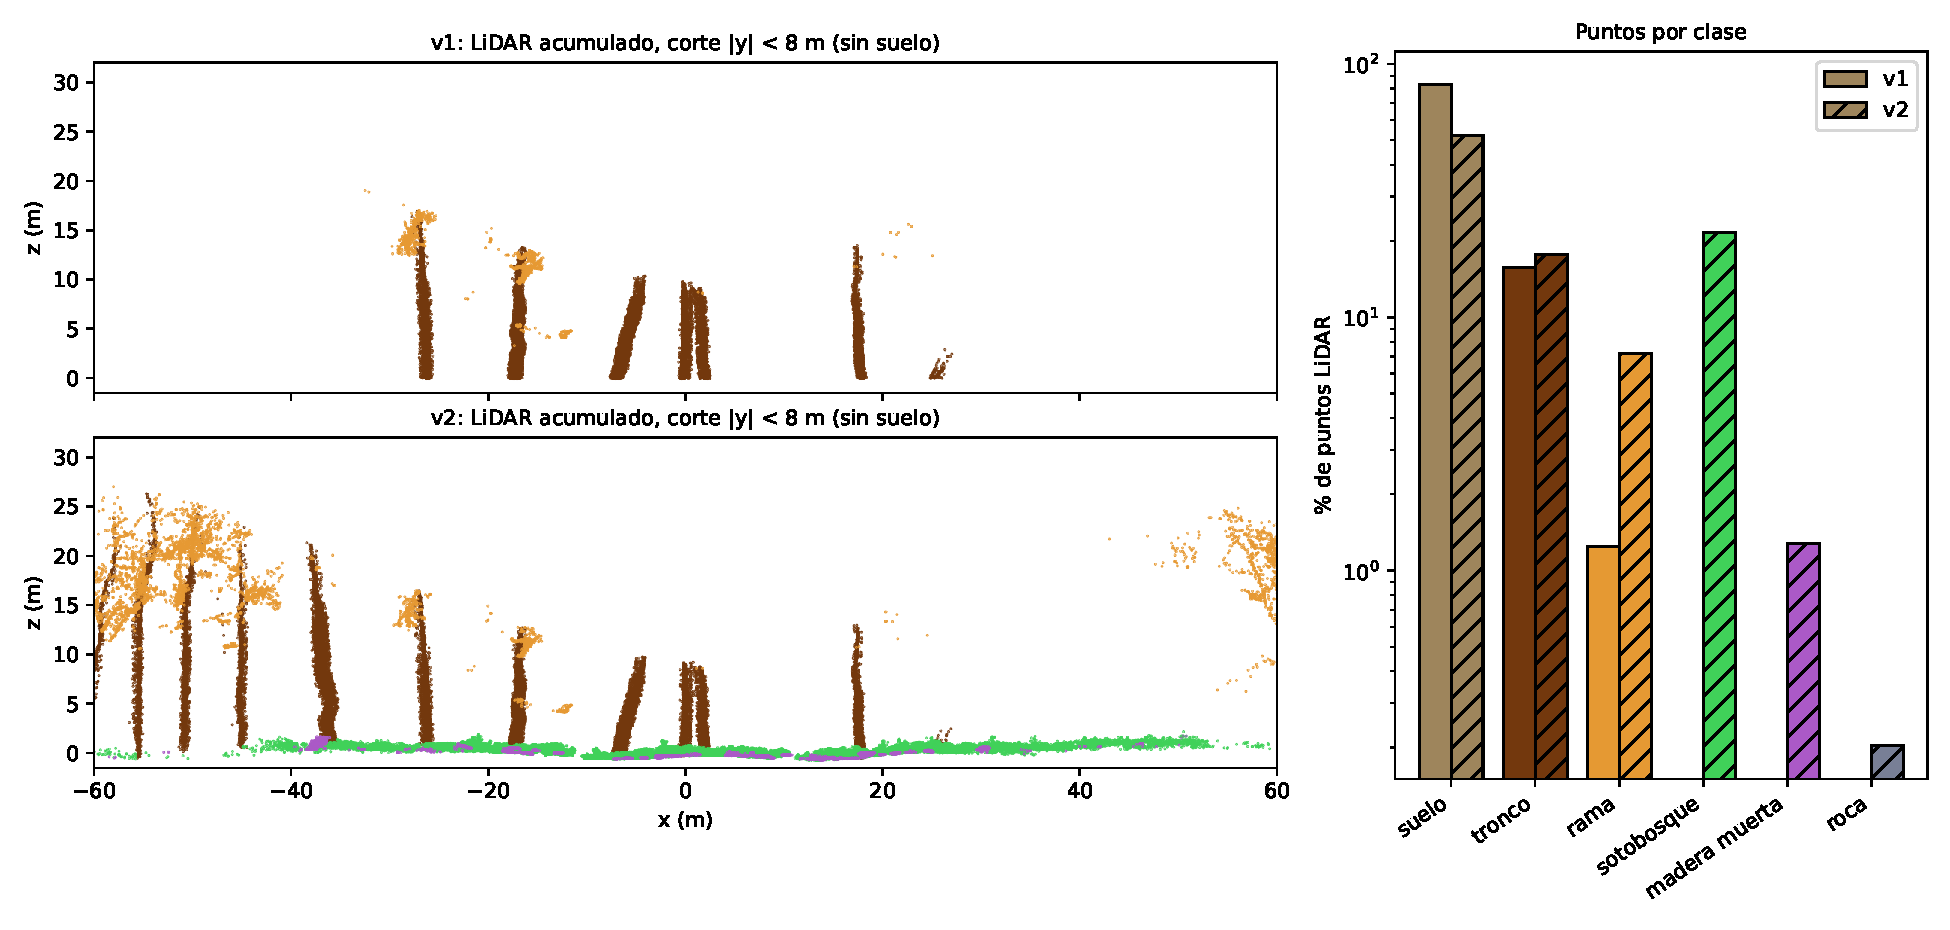
\includegraphics[width=\linewidth]{figs/lidar_v1_v2.pdf}
\caption{LiDAR Ouster OS1 simulado: corte lateral del mapa acumulado durante una vuelta (sin suelo) en v1 y v2, y porcentaje de puntos por clase (escala logarítmica).}
\label{fig:lidarv}
\end{figure}

\paragraph{Coherencia geométrica.} En ambas versiones el suelo medido por el LiDAR coincide con el terreno (error mediano de 1--4\,mm). Ningún objeto queda a menos de 1,7\,m del sensor, así que el recorrido está despejado. En v1, los puntos de tronco de cada árbol caen a una mediana de 0,25--1\,m de la posición de su base (hasta 2,7\,m en troncos inclinados).

\paragraph{Qué cambia con la ambientación.}
\begin{itemize}
  \item \textbf{Escena más compleja:} el sotobosque pasa a ser la segunda clase del LiDAR (21,7\,\%) y el suelo baja del 83 al 52\,\%. Una red entrenada en v1 nunca habría visto vegetación baja, que en un bosque real ocupa una parte importante del escaneo cerca del suelo.
  \item \textbf{Más copa visible:} la proporción de ramas sube de 1,3 a 7,2\,\%, sobre todo por las copas del anillo exterior, que el LiDAR ve a distancia. Desde dentro de la parcela, el campo vertical de $\pm21^\circ$ apenas alcanza las copas a 15--30\,m de altura.
  \item \textbf{Poca oclusión de troncos:} los 24 árboles de la parcela siguen viéndose en cada barrido, y los puntos de tronco por árbol solo bajan un 4\,\%, porque el sotobosque es bajo.
  \item \textbf{Coste:} v2 tarda un 36\,\% más en simularse y produce un 53\,\% más de datos.
\end{itemize}

% =====================================================================
\section{Discusión}

\paragraph{Escalera fidelidad--novedad.} Los resultados confirman una escalera clara: cuanto más se apoya un generador en geometría real, más fiel y menos novedoso es (G0 $\to$ G2 $\to$ G4), y los métodos sin datos reales (G5, G6) son fácilmente distinguibles. Esto coincide con lo que la literatura sugiere sobre la importancia de la diversidad~\cite{she2026scaling}. También indica que los generadores de gráficos por ordenador sin calibrar no deberían usarse como sustitutos de árboles tropicales reales. Siguen siendo útiles, sin embargo, como \emph{controles} de baja similitud para estudiar si el parecido predice la utilidad.

\paragraph{Por qué G4 funciona mejor que G5.} Ambos construyen árboles desde cero con información de la especie. La diferencia es que G4 conserva la distribución \emph{conjunta} de los rasgos de cada rama y condiciona por el grosor del padre, mientras que G5 muestrea rasgos independientes alrededor de su media. Esto ilustra la advertencia de que muestrear distribuciones marginales produce árboles raros aunque cada rasgo individual cuadre.

\paragraph{Limitaciones.}
\begin{itemize}
  \item Los rasgos se calculan sobre QSM, que son a su vez reconstrucciones con sesgos (por ejemplo, la regla de tubería de 1,34 y los huecos entre cilindros), no sobre los árboles reales.
  \item Con 49 árboles de \emph{test}, el \NNA{} tiene poca potencia estadística, así que \enquote{indistinguible} puede significar solo \enquote{pocos datos}.
  \item No se comprueban intersecciones entre ramas, y los árboles no tienen hojas.
  \item La alometría publicada de BCI~\cite{martinezcano2019allometry} no se pudo descargar porque el repositorio exige autenticación. Las reglas se ajustaron con nuestros datos de \emph{train}.
  \item En Isaac, la profundidad de la cámara es ideal (sin el ruido estereoscópico de una D455) y el LiDAR no modela la reflectancia del material de forma calibrada.
  \item En v2, el bosque que se ve al fondo de la cámara es la fotografía del cielo HDRI: no tiene geometría, así que aparece sin profundidad y etiquetado como fondo, y el LiDAR no lo ve. Para entrenar con la cámara conviene un cielo sin árboles o enmascarar el fondo.
  \item El sotobosque y la madera muerta son modelos genéricos (CC0), no especies medidas en BCI. La textura del suelo se repite visiblemente desde el aire.
  \item Todavía no hemos medido la utilidad de los sintéticos para entrenar redes.
\end{itemize}

% =====================================================================
\section{Conclusiones y trabajo futuro}

Implementamos y evaluamos ocho generadores de árboles tropicales sintéticos de las tres familias de la literatura con un protocolo que separa estrictamente \emph{train} y \emph{test}. La recombinación de ramas de la misma especie (G2) es la más fiel. El generador procedural que sortea reglas de ramas reales (G4) es el único que crea árboles realmente nuevos con fidelidad razonable. Su mezcla G2+G4 ofrece el mejor equilibrio. Con ella construimos un bosque virtual en Isaac Sim, en una versión solo con árboles y otra ambientada, con LiDAR y cámara RGB-D simulados que generan datos etiquetados por clase y se visualizan en tiempo real. La ambientación cambia sustancialmente la distribución de clases que ven los sensores.

Los siguientes pasos son:
\begin{enumerate}
  \item Entrenar redes de segmentación (suelo/tronco/rama) con datos reales, sintéticos (v1 y v2) y mixtos, y evaluarlas sobre las nubes reales de BCI (TSTR). Comparar v1 y v2 indicará cuánto aporta la ambientación.
  \item Comprobar si el \NNA{} de cada generador predice su utilidad.
  \item Añadir hojas~\cite{akerblom2018leaf}, aprendidas de las nubes reales de hoja de BCI, y compararlas con ellas (trabajo iniciado, fuera del alcance de este documento).
  \item Simular el escaneo terrestre real con HELIOS++~\cite{winiwarter2022helios} o con el LiDAR RTX colocado como en la campaña original.
  \item Ajustar G4 por modelado inverso~\cite{stava2014inverse} para corregir el reparto de volumen entre órdenes.
\end{enumerate}

\paragraph{Reproducibilidad.} El código, los scripts que regeneran todas las tablas y figuras de este documento y las instrucciones están en \url{https://github.com/Nosl3n/Synthetic_Tree_G}: \texttt{synth\_trees/} (generadores y evaluación) e \texttt{isaac\_forest/} (geometría, escenas v1 y v2, sensores y visor). Los datos de entrada son públicos~\cite{krishnamoorthy2022data}. Todas las semillas están fijadas: una ejecución desde cero en un entorno limpio reproduce bit a bit los 6\,080 árboles sintéticos y todas las métricas de las \cref{tab:res,tab:mix}. Las grabaciones de sensores, los videos y las escenas se distribuyen aparte por su tamaño.

\printbibliography[title={Referencias}]

\end{document}
